\documentclass[12pt]{report}
    \usepackage{blindtext}
    \usepackage{hyperref}
    \usepackage{tocloft}
    \usepackage{natbib}
    \usepackage{graphicx}
    % \usepackage[newfloat]{minted}
    \usepackage{caption}
    \usepackage{amsmath}
    \usepackage[table]{xcolor}
    \usepackage[a4paper, total={6in, 8in}]{geometry}
    \newenvironment{longlisting}{\captionsetup{type=listing}}{}
    \title{%
      GPT-2 Based Meme Generator\\~\\
      \large Final Year Project (CTEC3451) \\
        De Montfort University}
    \author{Artem Bobrov (P2547788)}
    \date{Jan 14 2021}
    \setlength{\parindent}{1em}
    \begin{document}
    \maketitle
    \thispagestyle{empty}
    \clearpage
    \tableofcontents
    \setcounter{tocdepth}{1}
    \thispagestyle{empty}
    \clearpage
    \section*{Abstract}
    \addcontentsline{toc}{section}{Abstract}
    
    \paragraph{}
    % Abstract text
    
    This project explores the possibilities of deep learning mechanisms to create and improve the ways of 
    social interaction in the 21st century. The main idea of the project is to prove that modern trained neural networks can 
    synthesise entertainment data based on the input, embedded in an application that is easy to use by every user.
    
    
    \section*{Literature Review}
    \addcontentsline{toc}{section}{Literature Review}
    \paragraph{}

    \subsection*{Introduction}
    \addcontentsline{toc}{subsection}{Introduction}
    \paragraph{}
    
    % Lit review for GPT-2 Backend (Python)

    GPT-2 introduces wide possibilities when it comes to human-like text synthesis. It is developed by OpenAI in February 2019 but the
    release to the public was postponed due to the apprehension that it could potentially be used to conduct malicious and harmful activities. The successor to
    the first GPT family member has been trained on a larger dataset and parameter count with around ten-fold growth. The reason behind
    choosing this exact neural network to produce this project lies in the philosophy followed by its creators. The aim was to take a new approach to the purpose of the system.
    The past neural networks "are better characterized as 'narrow experts' rather than  'competent generalists'" \citep{radford_wu_child_luan_amodei_sutskever_2019} and that was
    the main restraining factor. GPT neural network family uses transformer architecture with attention mechanism which allows faster training due to significantly increased parralelism \citep{attention_is_all_you_need}.
    There are several advantages of using transformer neural networks to process text when compared to convolutional and recurrent neural networks (CNN and RNN). Transformers deal with sentences within a text as a whole and not word by word.
    Self attention is another advantage of transformers since it allows to relate different positions of a single sequence (sentence) to calculate a representation of it \citep{attention_is_all_you_need}.
    And third major difference is positional embeddings. This concept allows the usage of fixed weights that encode information about a specific token in a sequence.
    Convolutional neural networks are very good at processing images and detecting patterns in them. Recurrent neural networks are mainly used in evolutionary robotics to deal with vision \citep{inproceedings}.
    
    
    \clearpage

    \subsection*{Transformer Neural Networks}
    \addcontentsline{toc}{subsection}{Transformer Neural Networks}
    \paragraph{}

    Transformer neural networks continue to gain more popularity among the other artificial intelligence systems for solving 'Natural Language Processing' problems.
    Before transformers gated recurrent units with added attention mechanism were mainly used to process natural language but transformers based on solely that attention mechanism
    has proven that they're more effiecient in solving particular problems \citep{attention_is_all_you_need}. A vast amount of them used encoder-decoder structure in which the encoder maps
    an input sequence of symbol representation to a sequence of continious representation. Using that continious representation the decoder generates an output sequence. Also it uses the
    already generated output as an additional input in order to learn and generate more accurate output.

    Encoder and decoder stacks consist of six identical layers. Every encoder layer has two sub-layers and every decoder layer has three sublayers. The first two sublayers of the decoder are 
    similar to the encoder sublayers. The first is a multi-head self-attention mechanism and the second is a fully connected feed-forward network. The third layer of the decoder works with the output
    of the encoder by performing multi-head attention over it.

    \begin{figure}[htbp]
        \centerline{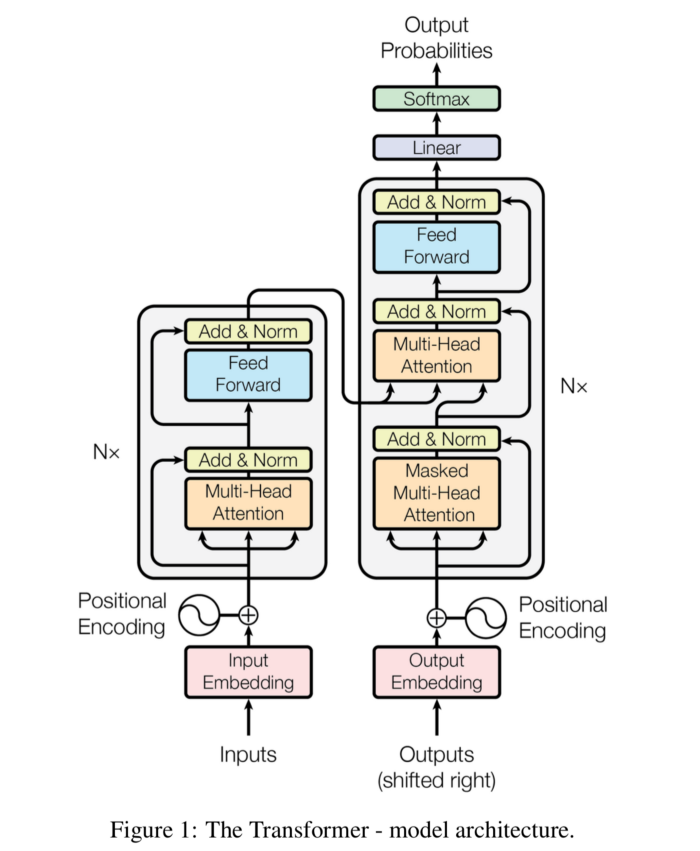
\includegraphics[scale=.35]{img/transformer_model.png}}
        \label{transformer_model}
    \end{figure}

    Since 2019 (release of GPT-2) a lot have changed in the field of transformers and as of November 2020 transformers are separated in different categories which different from each other in some aspects.
    Those categories are: Reformers, Linformers, Linear Transformers, Sinkhorn Transformers, Performers, Synthesizers, Sparse Transformers, and Longformers \citep{LRA_benchmark}. Using this LRA benchmark the
    efficiency of different transformer models could be measured and this could give a better understanding how and in what areas they should be used. This testing suite is available in Python and is open-source so
    everyone could build upon it.

    The suite developers pursued a goal of creating a suite for benchmarking having several important ideas in mind. Generality, Simplicity, Challenge, Long Inputs, Probing diverse aspects and accessibility of the suite.
    LRA Benchmark article depicts using a table of results for the comparison between different models. First test - Long 'ListOps' aims to test the parsing ability of the models and is a more complex version of the standard 'ListOps' task \citep{ListOps}.
    The best result is given by `The Reformer'. Other conducted tests can be seen in the table provided in the research paper. The average score of `Big Bird' is the highest, although it never showed best single result.

    \subsection*{Convoluational Neural Networks}
    \addcontentsline{toc}{subsection}{Convolutional Neural Networks}
    \paragraph{}

    Convolutional neural networks were introduced long before transformers and have been mainly used to analyse visual imagery \citep{VALUEVA2020232}. Also they've been proved to be able to undertake such tasks as recommender systems, natural language processing and financial time series.
    These networks are based on multilayer perceptron models but with implemented regularisation in order to avoid overfitting and that implies that multilayer perceptron neural networks are fully connected - each neuron of the previous layer is connected to every neuron in the next layer and that is the cause of overfitting.
    That problem has been solved with weight decay, which effectively is adding a penalty term to the cost function. This leads to weight shrinking in the backpropagation step, and trimming connectivity of a neural network which can be described as pruning - removing some unnecessary weights or neurons. Weight prunin is more popular than neuron because it's less likely
    to hurt network's performance and much easier to do. 

    The origin of the convolutional networks is the `neocognitron' introduced by a Japanese computer scientist Kunihiko Fukushima in year 1980 \citep{neocognitron}. It used two types of layers: convolutional layer and downsampling layer. The mechanism of interaction of these two types of layers is the following:
    Convolutional layer units whose receptive field cover previous layer. On the other hand downsampling layer units had receptive fields which covered the previous convolutional layers. The most popular method of training used for CNNs is backpropagation.

    Convoluational neural networks perform unbelievably well in image recognition, for example - recogntion of handwritten characters testing using MNIST database showed an amazing result of 0.23\% \citep{image_classification_article}.

    \subsection*{Recurrent Neural Networks}
    \addcontentsline{toc}{subsection}{Recurrent Neural Networks}
    \paragraph{}

    Recurrent neural networks have been derived from feedforward neural networks. They have internal state memory that allows them to work with long sequences of data. Everything that is sequential like connected handwriting or speech can be easily converted to digital format using RNNs \citep{rnn_article}.
    This type of networks is referred to as infinite impulse response class which can be applied not only to neural networks but to many other systems that produce an output based on an input which depends on time variable. 
    There are different architecture variants of RNNs - fully recurrent, Elman and Jordan networks, Recursive and one that marked a big growth in recurrent neural networks - `Long short-term memory' \citep{10.1162/neco.1997.9.8.1735}.
    LTSM networks showed a great performance in speech recognition, machine translation and other important areas \citep{ltsm_article}.

    LTSM also is a type of a recurrent neural network that happened to avoid `vanishing gradient problem'. The problem affects the training process and weight adjustment in particular. The standard training process of a neural network is performed in a number of steps:
    the error is updated accordingly every iteration and the weight are changed regarding the error value. The problem is encountered when the gradient is so small that it prevents the weights from changing. The opposite of the `vanishing gradient problem' is `exploding gradient problem' - the change in weights is too big \citep{vanishing_weight}.

    \subsection*{Applications of neural networks in entertainment}
    \addcontentsline{toc}{subsection}{Application of neural networks in entertainment}

    \subsubsection*{Introduction}
    \addcontentsline{toc}{subsubsection}{Introduction}
    \paragraph{}

    Since artificial intelligence systems, transformer neural networks in particular, are good in synthesising text that is nearly indistinguishable from human phrases - that allows to make a presumtption: are modern neural networks developed and trained enough to be used to generate
    entertainment short texts based on already created so known `memes'? It's important to understand the modern culture of internet and the heart of it - thematic pictures with short jokes written on them to undertake a project directly related to it.
    Memes can be found everywhere on the Internet nowadays and they constantly change and evolve. Their primary function is to entertain the community in a harmless way yet our society is very diverese and has different interests - that explains the existence of memes which can be used
    to "further political ideals, maginfy echo chambers and antagonise minorities" since it became a very popular communcation method \citep{dank_learning}. 


    %\subsubsection{How does it work?}
    %\addcontentsline{toc}{subsubsection}{How does it work?}
    %\paragraph{}

    %In order for a neural network to create a meme, there are several steps involved in that process. Given a training set of such images, the text from them should be recognised and stored using Python libraries such as `PyTesseract', then it should be fed to the neural network and then taken as a processed string
    %the generated text should be attached to the template of the meme from which it has been recognised. To attach a string to a picture - the preferred library is called `Pillow'.

    \subsubsection{Tesseract}
    \addcontentsline{toc}{subsubsection}{Tesseract}
    \paragraph{}

    `Tesseract' is an optical character recognition tool which can be both electronic or mechanical and is used to convert many types of text (handwritten, typed, printed etc.) to digital \citep{tesseract_article}. A plenty of systems use this tool to scan all kind of documents to store it digitally.
    Modern OCR is trained enough to work with different fonts, languages and even image recognition whereas early versions had to be fed with every character separetely.

    PyTesseract is a library written for Python which allows the usage of OCR functions directly in a program. This is vital for this project because the main source of data exists as images rather than plain text strings.

    \subsubsection{Pillow}
    \addcontentsline{toc}{subsubsection}{Pillow}
    \paragraph{}

    `Pillow' is a library for Python that explores vast possibilities when it comes to working with images. Initially the project was called PIL (Python Imaging Library) but then it was discontinued in 2011.
    Pillow is a successor of the first library and is still being updated. The latest stable version was released in April 2021. The author of the fork (a copy of a repository that is being managed by someone else rather than the creator of the original repository) has set several goals to follow when maintaining the product - continuous integration testing, publicised development activity and regular releases to Python Package Index \citep{pillow_about}. 
    It is capable of manipulating images in a variety of ways but one of the most important features of this library that will be used in this project is: "Adding text to an image".

    \subsubsection*{PyTorch or TensorFlow?}
    \addcontentsline{toc}{subsubsection}{PyTorch or TensorFlow?}
    \paragraph{}

    PyTorch and Tensorflow are both tools for working with neural networks and offer different advantages and disadvantages. They both allow utilising your GPU's power in order to train NNs on big datasets. Any of these frameworks can be used to create an architecture of a neural network but they have some differences.
    GPU processing in PyTorch is implemented using CUDA system created and maintained by NVIDIA while TensorFlow uses its own algorithms which may affect the performance of the training. One of the main features that is implemented in PyTorch is data parallelism. PyTorch makes it automatically while TensorFlow should be manually given an instruction.
    Tensorflow's functionality is more extensive but requires more effort to create something.

    In the long run, there are many implemented tools based on PyTorch or TensorFlow which can be used to overcome the difficulties of reinventing the wheel. Some which are located on GitHub are available open-source to the community.

    \subsection*{Conclusion}
    \addcontentsline{toc}{subsection}{Pillow}
    \paragraph{}

    Summing up everything that has been stated before, nowadays the interest towards neural networks and other artificial intelligence systems grows with exponential speed. Literature available online that is crucial to familiarise yourself with when working on such a project is extensive and allows more in-deep research to be carried out. Having that in mind, writings about AI are more inclined towards scientific purposes rather than entertainment.
    There are many types of neural networks available open-source: Recurrent Neural Networks, Convolutional Neural Networks, Perceptrons, Transformers etc. Transformers are the best choice when it comes to entertainment and text generation in particular, since they use attention mechanism - it greatly reduces training times. GPT-2 has a major training base of 1.5 billion parameters compared to BERT's two versions: 110 million and 340 million parameters (as of 2019). It makes GPT-2 a winner in more accurate text synthesis.


    
    \section*{System Design}
    \addcontentsline{toc}{section}{System Design}

    \subsection*{System UI (frontend)}
    \addcontentsline{toc}{subsection}{System UI (frontend)}
    \paragraph{}

    The main key of the system UI when it aims to hold a `dialogue' with the user is simplicity. The system can include a lot of parameters, functions, features which will be implemented in an outstanding way but if it fails to correctly introduce these features to the user and they become convoluted - it's a problem.
    
    \paragraph{}

    \begin{figure}[htbp]
        \centerline{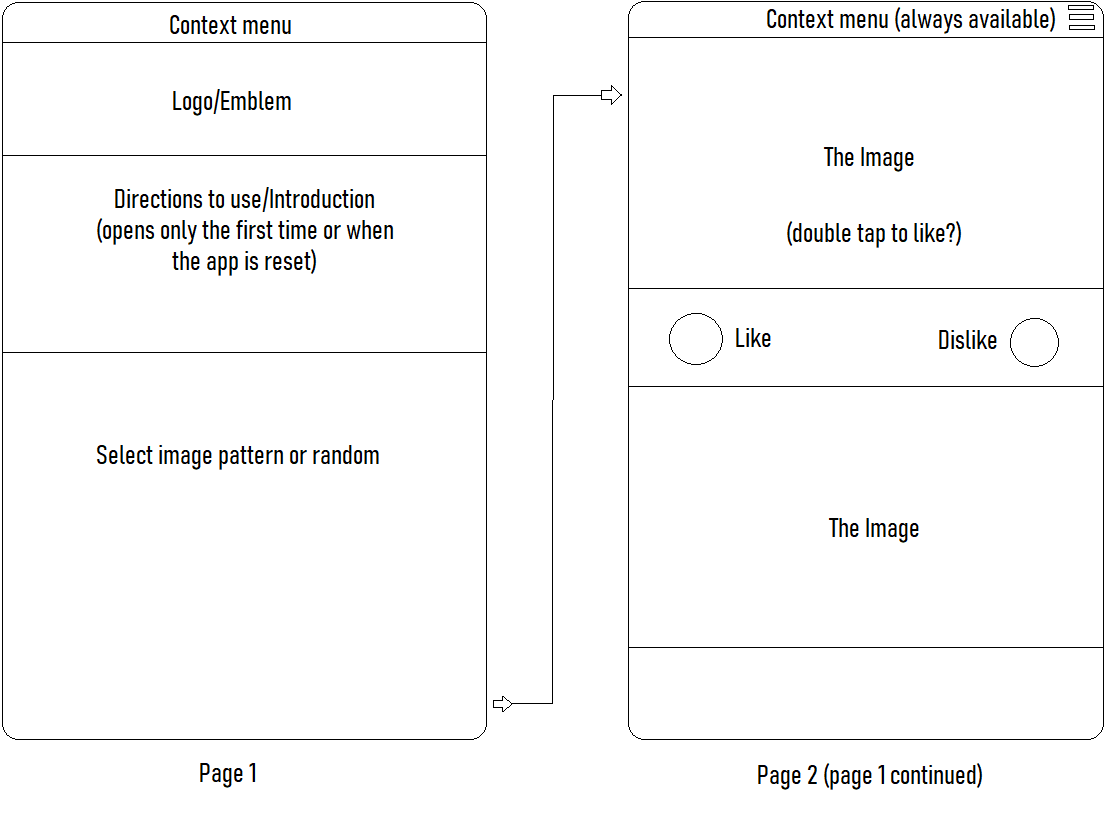
\includegraphics[scale=.5]{img/system_ui.png}}
        \label{system_ui}
        \caption{Main page design}
    \end{figure}

    The ladning page features a simple approach to the design. In the beginning we have a context menu which will contain drop-down boxes to control the behaviour of the program which will be used to tailor the experience that suits the end user. It's planned the menu to contain settings to control the environment - change
    the appearence of the app, switch to another section (meme pattern), reload the app (in case of an emergency). 

    Next section of the interface is `Branding'. The app shouldn't only be practical but also has a decent appearence. The logo should match to overall design of the program and to complement it.

    `Directions to use' shows the user how to get the most out of the app and have a good experience. It will be shown only once on startup not to bother the user too much.

    `Select image' section will allow the user to select the beloved meme pattern on which will be based the generation of the future memes shown. If the user doesn't have a preferred pattern or just wants to watch all kinds of memes - random generation will be available as an option (it will be set automatically, if no input collected).

    The philosophy of the whole user interface which will be used in this project is to make the experience continious. Loading different pages manually is in the past, the modern idea of a scroller app is to make the usage seamless. Although the devices nowadays are very powerful and capable of handling massive amounts of calculations, it's still
    important to implement a good optimisation to make the usage of the app pleasant to the highest number of people. To balance somewhere in between experience and optimisation - `lazy loading' is the answer. The main idea is to move away from separate pages and implement everything combined in one long page which will be loaded consequentially and automatically when the user reaches the end of the `page'.

    Also as can be seen on the diagram above, every picture (meme) should have several buttons to express opinion. This can be achieved by using typical `like-dislike' system. To make even easier for the user to give positive feedback a double click system on the image can be used.
    
    \clearpage

    \subsection*{Interaction between frontend and backend}
    \addcontentsline{toc}{subsection}{Interaction between frontend and backend}

    \begin{figure}[htbp]
        \centerline{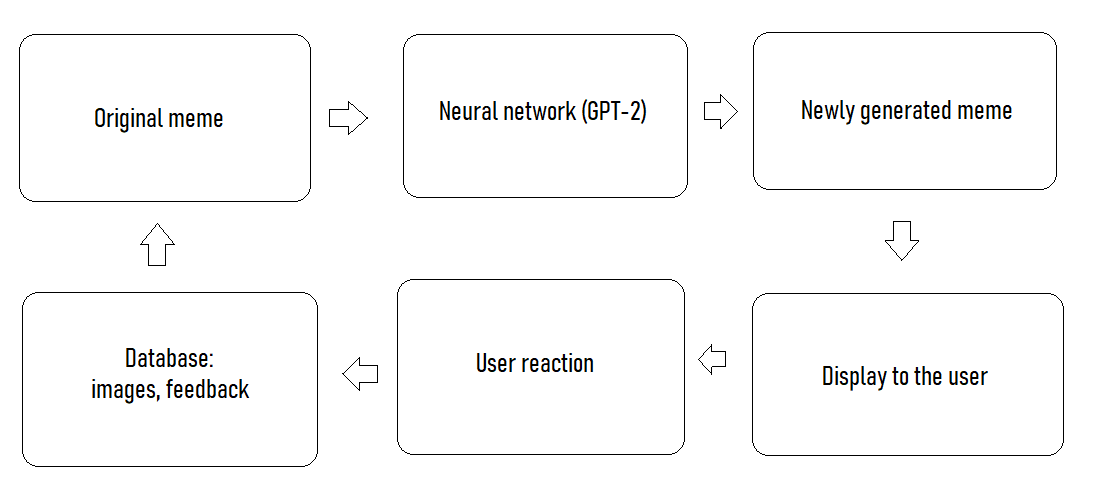
\includegraphics[scale=.5]{img/flow_diagram.png}}
        \label{flow_diagram}
        \caption{The system design flow chart}
    \end{figure}

    As can be seen on this figure the process involved in generating and showing the images is continous. First comes the database which will contain images and user reactions to each image. Reactions will be stored as a mass, not individual data. This will allow to understand better what the users like the most and what they don't. 
    The program will take the initial image, separate the text from it, remember what the image was, feed the text to the neural network and combine the output from the neural network and the existing image into a freshly generated meme. After that comes the process of displaying the image. Then the user, if they wish, can leave feedback. The loop repeats.

    The main bridge between backend and frontend in this project is the Python library called `Eel' \citep{eel_github}. It is similar to JavaScript's `Electron' and allows to code the frontend with a stack of HTML, CSS and JavaScript having Python in the backend. There is another library which is heavier and therefore has a higher entry level - `cefpython'.
    `Eel' makes possible linking buttons created using HTML/CSS to Python-implemented functions. This methodology is called `Function Exposure' \citep{eel_github}. Functions from Python could be exposed to JavaScript environment and vice versa.

    \clearpage

    \subsection*{Backend design}
    \addcontentsline{toc}{subsection}{Backend design}
    \paragraph{}

    \begin{figure}[htbp]
        \centerline{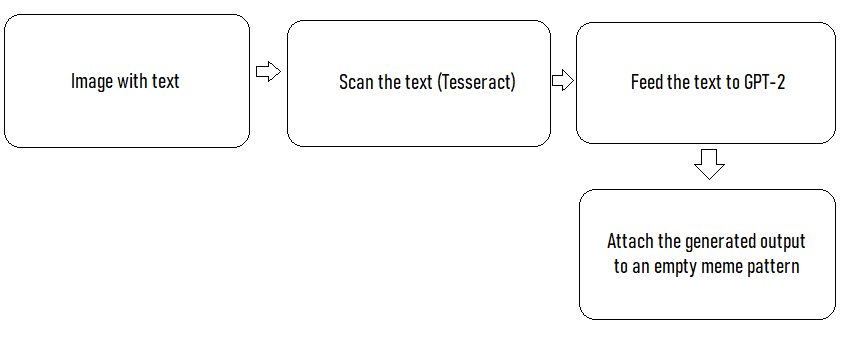
\includegraphics[scale=.5]{img/backend_diagram.png}}
        \label{backend_diagram}
        \caption{Backend design}
    \end{figure}

    The backend of the project is going to be implemented using Python programming language due to the availability of different frameworks and libraries. In the backend the process of the scanning the text from the image will be undertaken by a library called `PyTesseract' which allows the optical character recognition to be used in an optimised way.
    Next step of the backend process is to push the string to the neural network allowing it to use its massive database to synthesise similar text. Afterwards comes the process of attaching the generated output to an image. It is done using a tool called `Pillow' and it's aim is to work with all kind of images. The string will be styled to fit the pattern appropriately.

    \clearpage

    \section*{Functional Requirements}
    \addcontentsline{toc}{section}{Functional Requirements}
    \paragraph{}

    The function requirement report will join the early described diagrams in a whole idea. Figure 4 shows the relationship between the user and the developer and how this interaction will enhance the experience of the user.

    \begin{figure}[htbp]
        \centerline{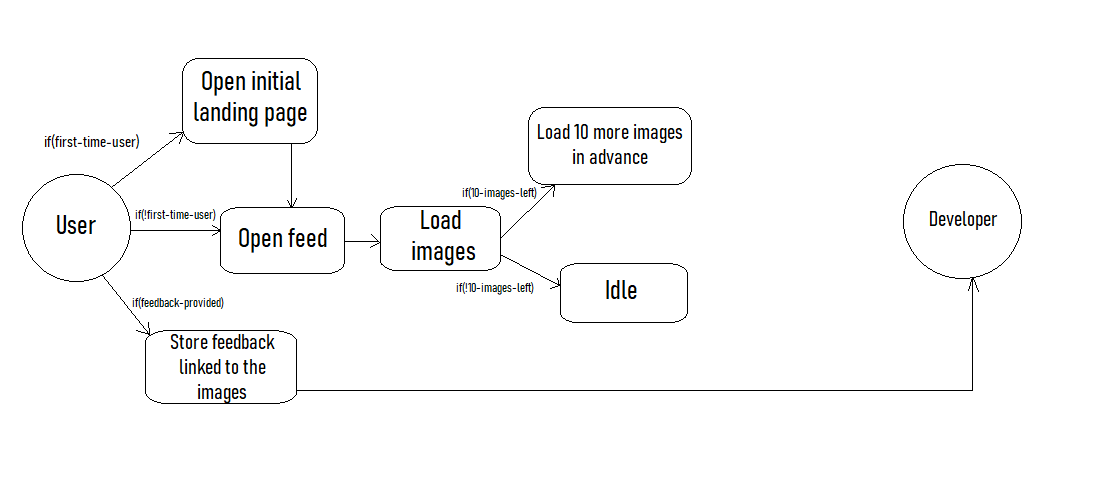
\includegraphics[scale=.5]{img/use-case-diagram.png}}
        \label{use_case_diagram}
        \caption{Use Case Diagram}
    \end{figure}

    The user has a way to communicate with the developer - hold a dialog in a non-verbal manner and explain what they like. This leads the system to be implemented in a `prosumer' way. The user not only consumes the content but also influences it. 
    The diagram explains different elements of the system and how they work together. Although the user has only one way to interact with the program, the program collects non-sensitive data about the user and decides which path to take. The `use case diagram' is not final and may be changed throughout the development.

    \clearpage

    \begin{table}[h]
        \centering
        \resizebox{\columnwidth}{!}{%
            \begin{tabular}{|lllll|}
                \hline
                \multicolumn{5}{|c|}{Overview}                                                                                                                                                 \\ \hline
                \multicolumn{1}{|l|}{Title}          & \multicolumn{4}{l|}{Scroll Example}                                                                                                     \\ \hline
                \multicolumn{1}{|l|}{Description}    & \multicolumn{4}{l|}{The user logs in to the app and scrolls down in order to see images}                                                \\ \hline
                \multicolumn{1}{|l|}{Actors}         & \multicolumn{4}{l|}{User}                                                                                                               \\ \hline
                \multicolumn{1}{|l|}{Pre-Conditions} & \multicolumn{4}{l|}{First time login, no preferred image pattern selected}                                                              \\ \hline
                \multicolumn{5}{|c|}{Basic Flow}                                                                                                                                               \\ \hline
                \multicolumn{1}{|l|}{Step 1}         & \multicolumn{4}{l|}{Run the script to check the boolean variable for first login}                                                       \\ \hline
                \multicolumn{1}{|l|}{Step 2}         & \multicolumn{4}{l|}{Show the welcome/landing page with short, simple instructions}                                                      \\ \hline
                \multicolumn{1}{|l|}{Step 3 (1/2)}   & \multicolumn{4}{l|}{As the user scrolls down - generate new images, when the user reaches last 10 items (pre-generation to avoid lags)} \\ \hline
                \multicolumn{1}{|l|}{Step 3 (2/2)}   & \multicolumn{4}{l|}{If the user doesn't reach to last 10 images - idle}                                                                 \\ \hline
                \multicolumn{1}{|l|}{Step 4}         & \multicolumn{4}{l|}{Unload the images that are far behind to decrease the load on the system}                                           \\ \hline
                \multicolumn{1}{|l|}{Step 5}         & \multicolumn{4}{l|}{As the user likes or dislikes some images - store the reaction linked to a certain image as statistical data}       \\ \hline
                \multicolumn{5}{|c|}{Post Condition}                                                                                                                                           \\ \hline
                \multicolumn{1}{|l|}{Condition 1}    & \multicolumn{4}{l|}{The app saved the data about user login}                                                                            \\ \hline
                \multicolumn{1}{|l|}{Condition 2}    & \multicolumn{4}{l|}{Adjusted settings saved - will be used on next login}                                                               \\ \hline
            \end{tabular}%
        }
        \caption{Use Case Specification}
    \end{table}

    The table above illustrates an example of using the application. Although, the program is not time-dependant (the user should be in control of what happens) and follows user's instructions, an attempt was made to adapt the flow of the actions in a time-dependant chart.
    The example is very simple and doesn't represent the whole potential of the app. One possible linear way is introduced in this table.

    \section*{Indicative Test Plan}
    \addcontentsline{toc}{section}{Indicative Test Plan}
    \paragraph{}

    \section*{Implementation Report}
    \addcontentsline{toc}{section}{Implementation Report}
    \paragraph{}

    The approach chosen to develop this project is FDD - Feature-driven development. Features are implemented first and then the unit tests will be written to prove that these features work correctly. The whole idea of the project is to prove that neural networks can create memes that are interesting to people.

    The current state of the development has the frontend and backend partly implemented. As of now the frontend features the ability to test the backend efficiently without writing unit tests. It visually shows what works and what doesn't. Content loading of the image stream when the user scrolls down is implemented using a `Load More' button powered by jQuery. The app has a branding and instruction screen but since the backend is only partly implemented - the app doesn't store information about users and wether they're using it for the first time.
    In the backend some functions that process images are fully implemented. For example, functions that scan the text and add it to the images work but they have to be enhanced. Reading the text from the image sometimes collects non-existent characters and some kind of a filter should be implemented that will throw away useless characters. On the other hand the code that adds the text to the image works perfect.

    For the frontend it's planned to implement 'lazy loading' using either React or jQuery and load the images from the database endlessly. 
    For the backend the main target is to adapt GPT-2 code and use it to process text.

    \addcontentsline{toc}{section}{Bibliography}
    \bibliography{reference}{}
    \bibliographystyle{agsm}

\end{document}